\chapter{Conception}
\label{chap:conception}

\section*{Introduction}
\addcontentsline{toc}{section}{Introduction}

Ce chapitre présente les choix de conception retenus pour répondre aux besoins identifiés au chapitre précédent : architecture générale du système, choix technologiques, puis modélisation détaillée (classes, séquences) des mécanismes centraux de la plateforme.

\section{Architecture générale}

Contrairement à une architecture en microservices distincts que l'on aurait pu envisager \emph{a priori} pour un tel système, la plateforme est conçue comme un \textbf{monolithe applicatif unique} (\emph{ai-core}) exposant l'ensemble des fonctionnalités métier via une API REST, consommé exclusivement par le backoffice. Ce choix, hérité de la version initiale du projet et confirmé pendant la phase de conception, se justifie par la taille de l'équipe (un stagiaire) et par la simplicité opérationnelle qu'il procure : un seul processus à déployer et à superviser, une seule base de données à administrer, sans les coûts de coordination (cohérence transactionnelle inter-services, observabilité distribuée) qu'imposerait une décomposition en microservices à ce stade de maturité du produit.

Le \emph{ai-core} est le \textbf{seul composant autorisé à accéder directement à la base de données PostgreSQL} : cette contrainte est imposée par l'architecture (le backoffice ne détient aucun identifiant de connexion à cette base) et non laissée à la seule discipline des développeurs. Le backoffice Laravel/Filament, à l'inverse, n'a d'autre moyen d'obtenir ou de modifier une donnée que d'appeler l'API REST du \emph{ai-core}.

\begin{figure}[h]
    \centering
    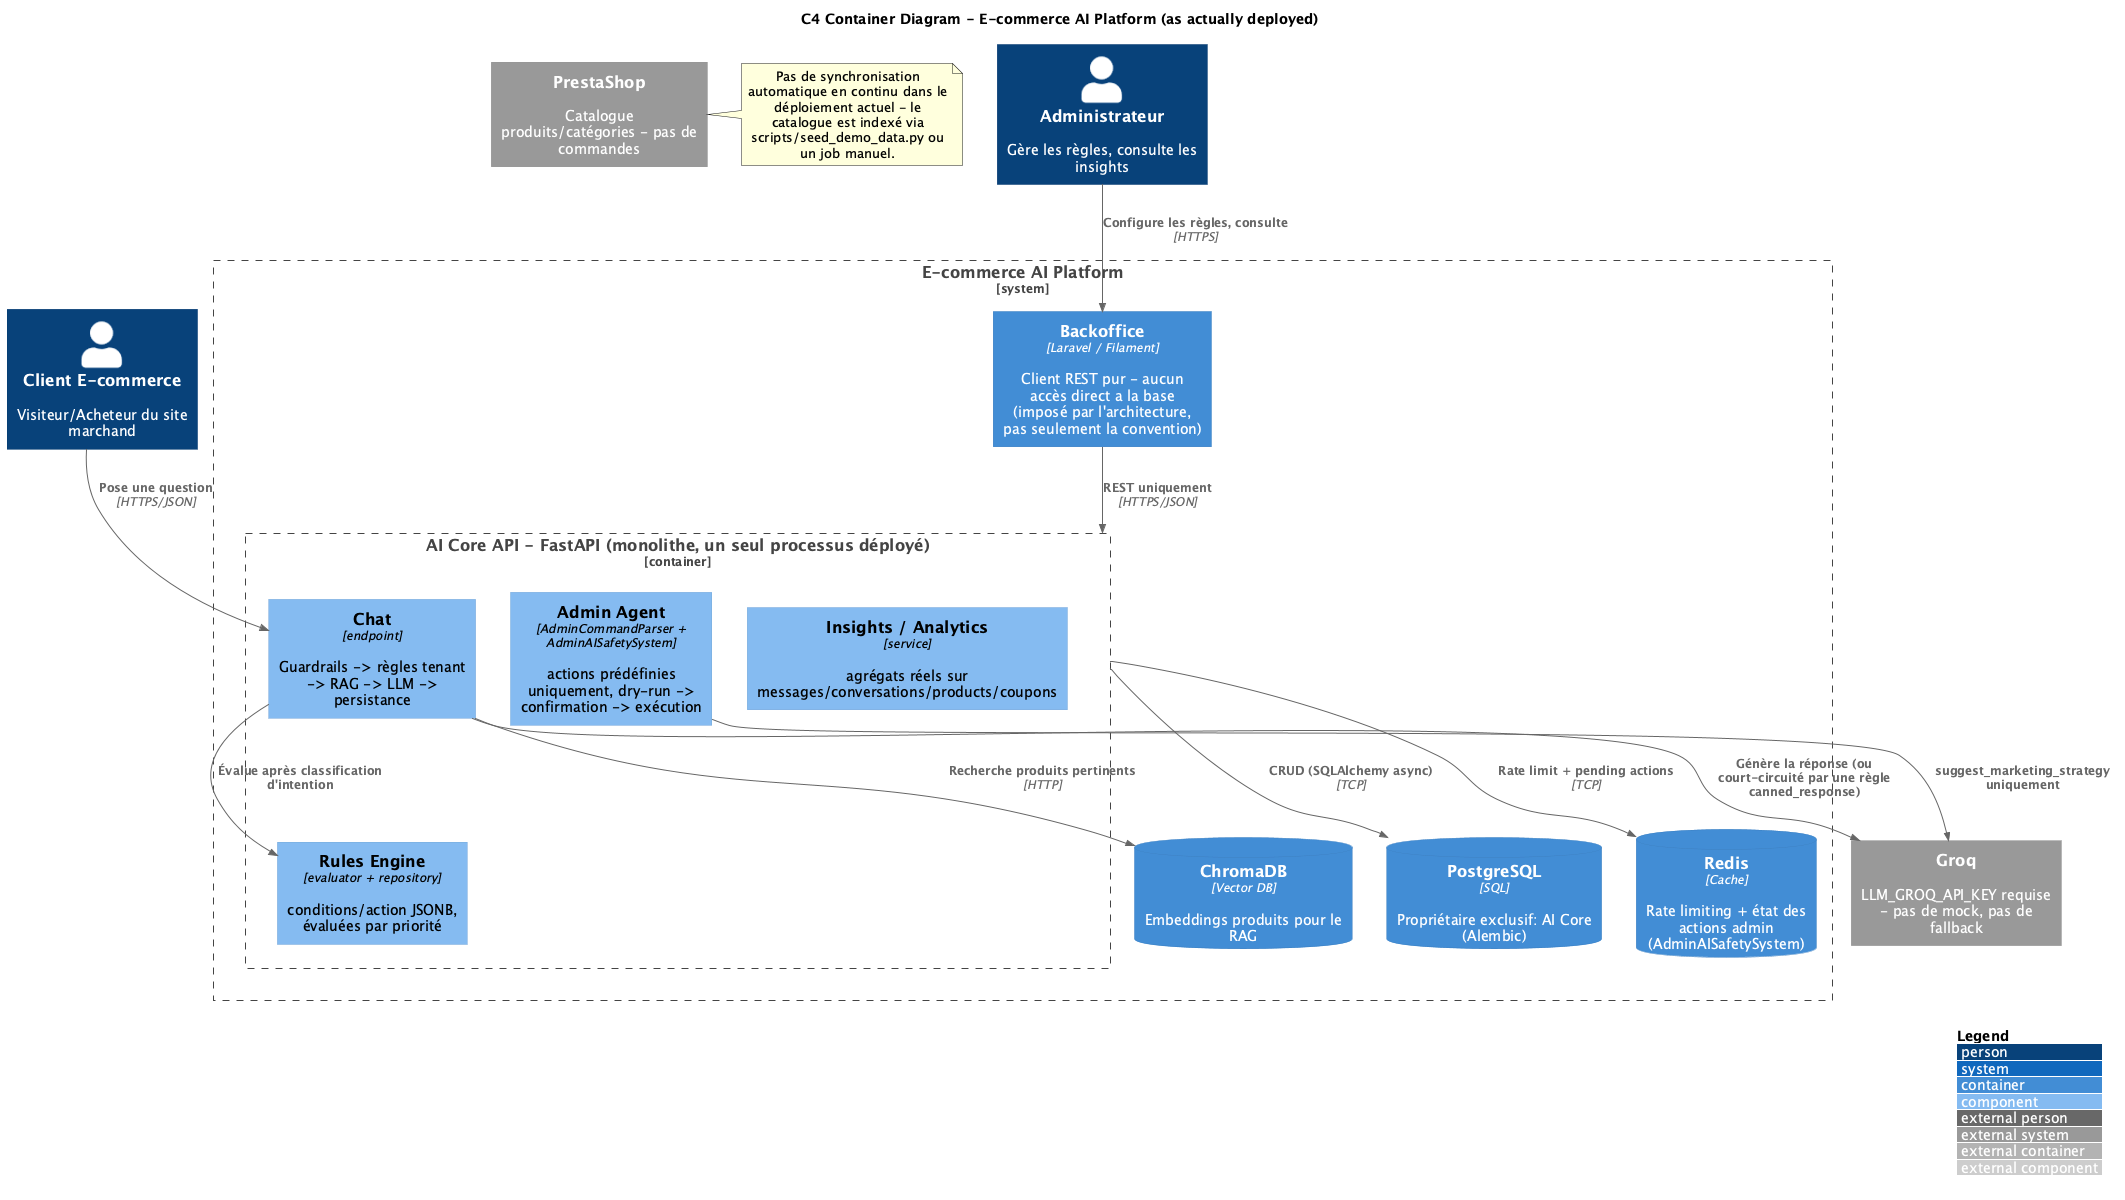
\includegraphics[width=\textwidth]{../diagrams/C4_Container.png}
    \caption{Diagramme de conteneurs (C4, niveau 2) de la plateforme}
    \label{fig:c4-container}
\end{figure}

Comme l'illustre la \cref{fig:c4-container}, quatre composants internes structurent le \emph{ai-core} : le \textbf{chat} (orchestration garde-fous -> règles -> RAG -> LLM -> persistance), le \textbf{moteur de règles}, l'\textbf{agent d'administration}, et le service d'\textbf{analyse de la demande} (\emph{insights}). Trois dépendances externes complètent l'architecture : \textbf{PostgreSQL} (persistance relationnelle, propriété exclusive du \emph{ai-core}), \textbf{ChromaDB} (base vectorielle pour la recherche sémantique de produits) et \textbf{Redis} (limitation de débit et état des actions d'administration en attente de confirmation).

\section{Choix technologiques}

\begin{table}[h]
\centering
\caption{Principaux choix technologiques}
\label{tab:stack}
\begin{tabular}{@{}p{3.5cm}p{4cm}p{6.5cm}@{}}
\toprule
\textbf{Composant} & \textbf{Technologie} & \textbf{Justification} \\
\midrule
API backend & Python 3 / FastAPI & Framework asynchrone performant, typage fort via Pydantic, génération automatique du schéma OpenAPI \\
Accès aux données & SQLAlchemy 2.0 (async) + Alembic & ORM mature avec support natif de l'asynchrone, migrations versionnées \\
Base relationnelle & PostgreSQL & Support natif du type JSONB, utilisé pour les conditions/actions des règles et les métadonnées des messages \\
Recherche sémantique & ChromaDB & Base vectorielle simple à opérer en conteneur, suffisante pour un catalogue produits de taille modérée \\
Cache / état transitoire & Redis & Nécessaire pour que l'état des actions d'administration en attente de confirmation survive aux redémarrages et soit partagé entre workers \\
Backoffice & Laravel 13 / Filament 3 & Productivité élevée pour construire une interface d'administration (CRUD, tableaux de bord) sans développer un frontend dédié \\
Interactivité backoffice & Livewire 3 & Composants réactifs côté serveur, cohérent avec l'écosystème Filament \\
Conteneurisation & Docker / Docker Compose & Environnement de développement reproductible, aligné sur le déploiement cible \\
Intégration continue & GitHub Actions & Exécution automatisée des tests et de l'analyse de qualité à chaque évolution \\
\bottomrule
\end{tabular}
\end{table}

\section{Modélisation du domaine}

Le diagramme de classes de la \cref{fig:class-diagram} présente les principales classes du système, regroupées par responsabilité : les entités du domaine persistées en base, le moteur de règles, l'agent d'administration, le service d'analyse de la demande, la couche de sécurité et l'infrastructure (fournisseurs de modèle de langage, recherche vectorielle, unité de travail transactionnelle).

\begin{figure}[h]
    \centering
    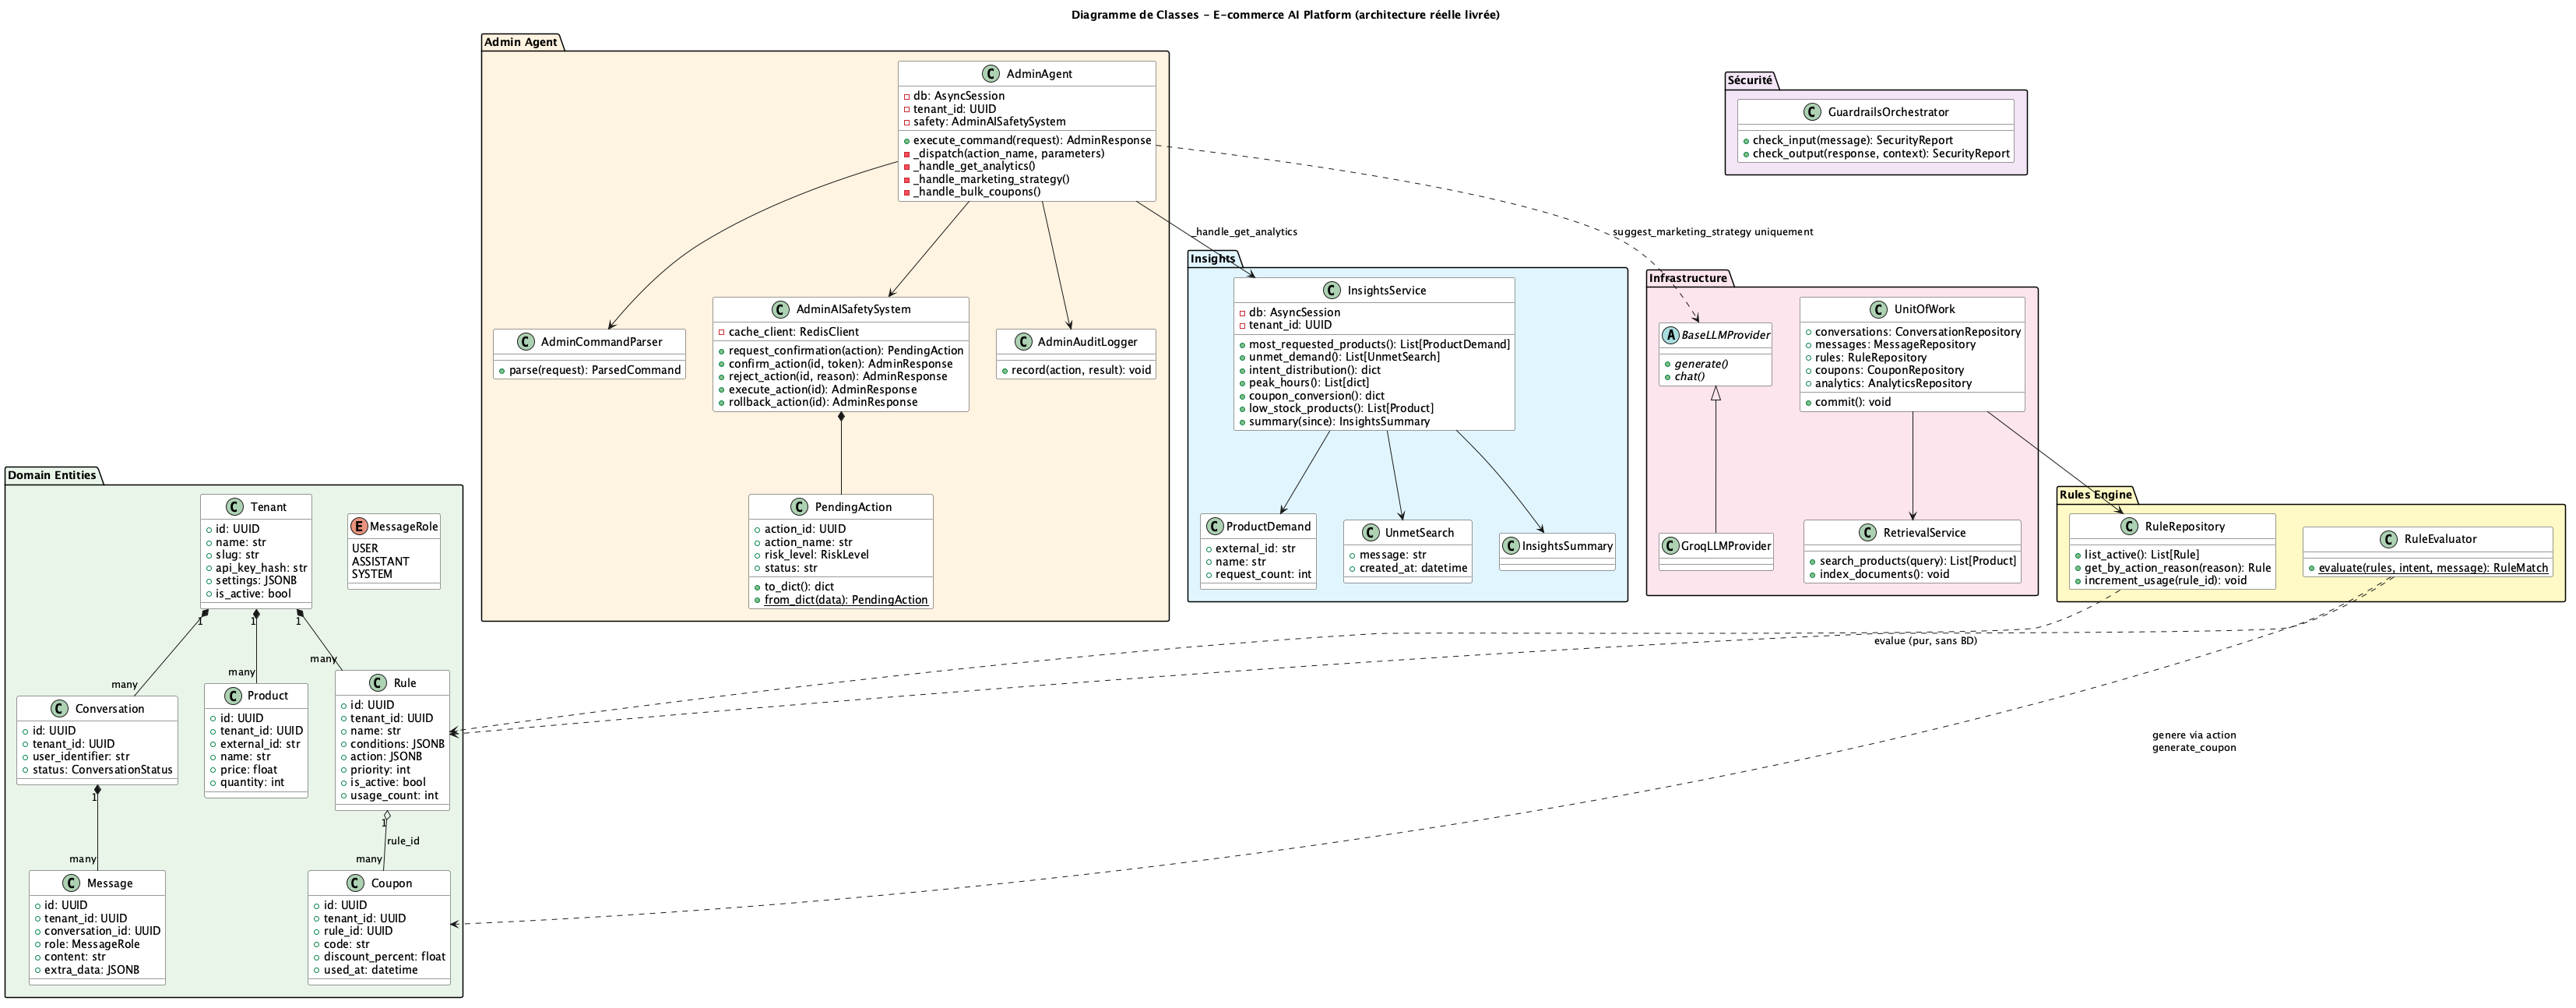
\includegraphics[width=\textwidth]{../diagrams/Class_Diagram.png}
    \caption{Diagramme de classes de la plateforme}
    \label{fig:class-diagram}
\end{figure}

Deux choix de conception méritent d'être détaillés, car ils ont directement découlé des contraintes identifiées au chapitre précédent.

\subsection{Le moteur de règles}

Le moteur de règles repose sur la séparation stricte entre \textbf{accès aux données} (\texttt{RuleRepository}, qui charge les règles actives d'un tenant, triées par priorité) et \textbf{évaluation} (\texttt{RuleEvaluator}, une fonction pure sans accès base de données ni effet de bord). Une règle est définie par des \emph{conditions} (intention détectée, présence d'au moins un mot-clé parmi une liste, ou présence de tous les mots-clés d'une liste) et une \emph{action} de l'un des trois types suivants : \texttt{canned\_response} (réponse préétablie, court-circuitant l'appel au modèle de langage), \texttt{inject\_instruction} (instruction ajoutée au contexte système envoyé au modèle) ou \texttt{generate\_coupon} (génération d'un coupon réel après la réponse). Le détail de ce mécanisme est illustré au \cref{chap:realisation} par le diagramme d'activités de la \cref{fig:rules-flow}.

Cette séparation permet de tester exhaustivement la logique de correspondance des règles sans base de données (voir \cref{chap:tests}), tout en gardant la persistance et les effets de bord (incrémentation du compteur d'utilisation, génération du coupon) dans la couche appelante.

\subsection{L'agent IA d'administration}

Le choix le plus structurant de ce chapitre concerne l'agent d'administration. Une architecture préexistante mais jamais réellement instanciée proposait un agent générique (\texttt{BaseAgent}) reposant sur des services partagés (\texttt{LLMGateway}, \texttt{RAGService}) eux-mêmes non testés et dépourvus de tout mode simulé, ce qui rendait cette voie coûteuse à finaliser sans bénéfice architectural clair. La décision retenue -- après comparaison explicite des deux options avec l'encadrant -- a été de \textbf{reconstruire l'agent d'administration sur les briques déjà éprouvées du système} : le fournisseur de modèle de langage utilisé par le chat (Groq, sans mode simulé -- les tests automatisés s'appuient sur un double de test isolé, jamais atteignable en développement ou en production), le service d'analyse de la demande, et un système de sécurité dédié.

Ce système de sécurité, \texttt{AdminAISafetySystem}, restreint l'agent à un ensemble fermé d'actions prédéfinies (\texttt{ACTION\_DEFINITIONS}), chacune associée à un niveau de risque (faible, moyen, élevé, critique) déterminant le circuit de validation requis : simple confirmation pour un risque moyen, double confirmation avec délai obligatoire pour un risque élevé, mise en file d'attente d'approbation humaine pour un risque critique. Ce workflow -- exécution à blanc (\emph{dry-run}), confirmation, exécution, annulation -- est illustré en détail par le diagramme de séquence de la \cref{fig:seq-admin-coupon}, pris sur l'exemple concret de la génération de coupons en masse.

\begin{figure}[h]
    \centering
    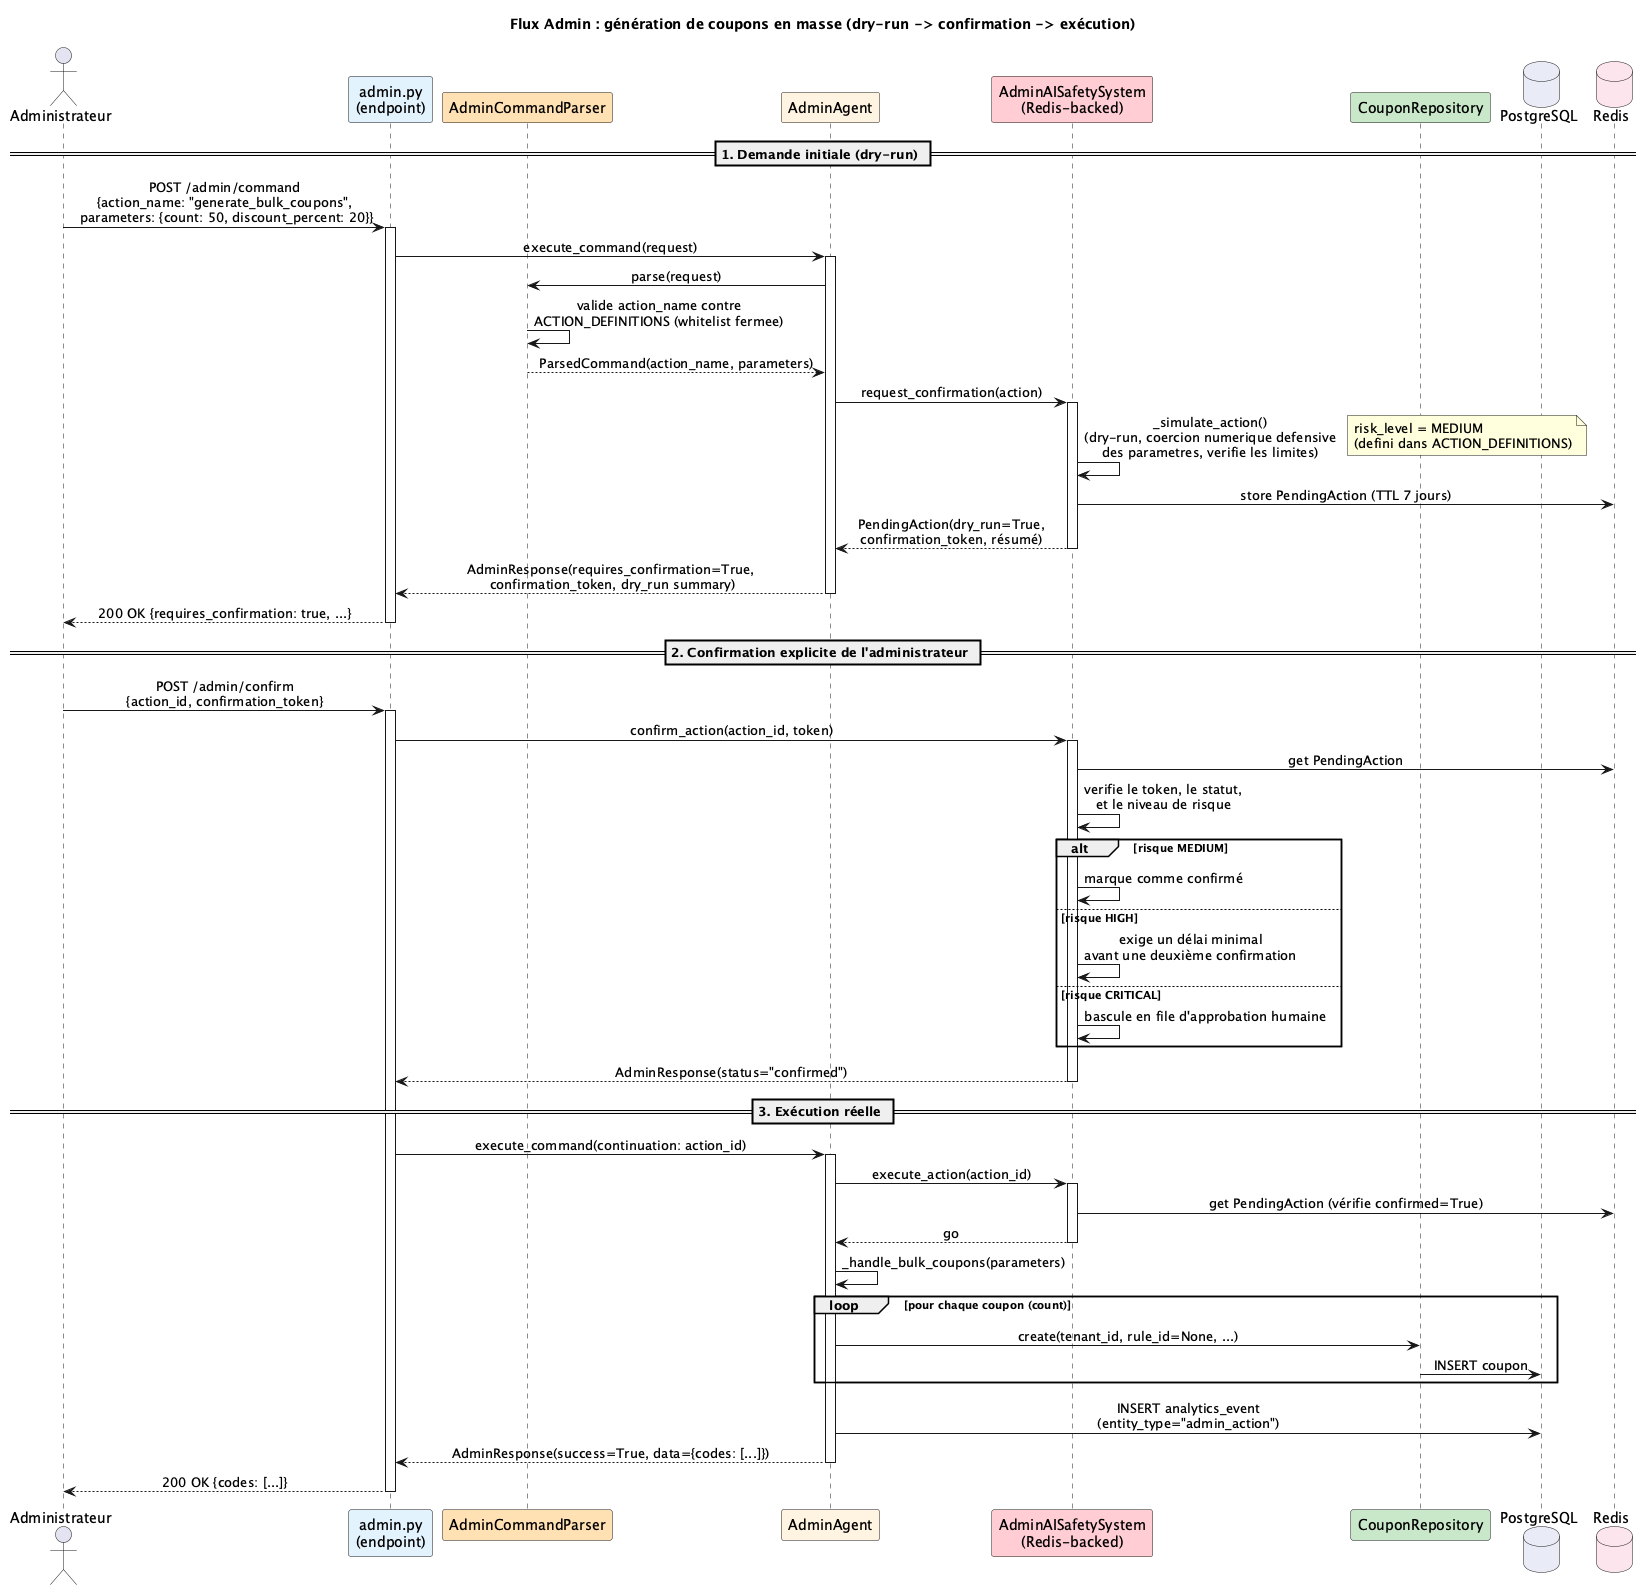
\includegraphics[width=\textwidth]{../diagrams/Sequence_Admin_Coupon.png}
    \caption{Séquence : génération de coupons en masse par l'agent d'administration}
    \label{fig:seq-admin-coupon}
\end{figure}

Point de conception notable : l'état des actions en attente de confirmation devait initialement être porté par Redis, mais l'implémentation héritée le maintenait en réalité dans un simple dictionnaire Python en mémoire -- ce qui aurait rendu toute confirmation invalide après un redémarrage du service, ou incohérente entre plusieurs \emph{workers} applicatifs. Ce point a été corrigé pendant la phase de réalisation (voir \cref{chap:realisation}, Sprint 5) en implémentant le stockage réel dans Redis, avec dégradation explicite en mémoire lorsqu'aucun client de cache n'est fourni (utile pour les tests unitaires existants).

\section{Séquence du chat conversationnel}

La \cref{fig:seq-chat} détaille le cheminement complet d'un message client, de sa réception à la persistance de la réponse : validation par les garde-fous de sécurité en entrée, classification de l'intention, évaluation des règles métier du tenant, puis -- selon le résultat -- court-circuit par une réponse préétablie, ou poursuite vers la recherche vectorielle de produits (RAG), l'appel au modèle de langage et la validation des garde-fous en sortie.

\begin{figure}[h]
    \centering
    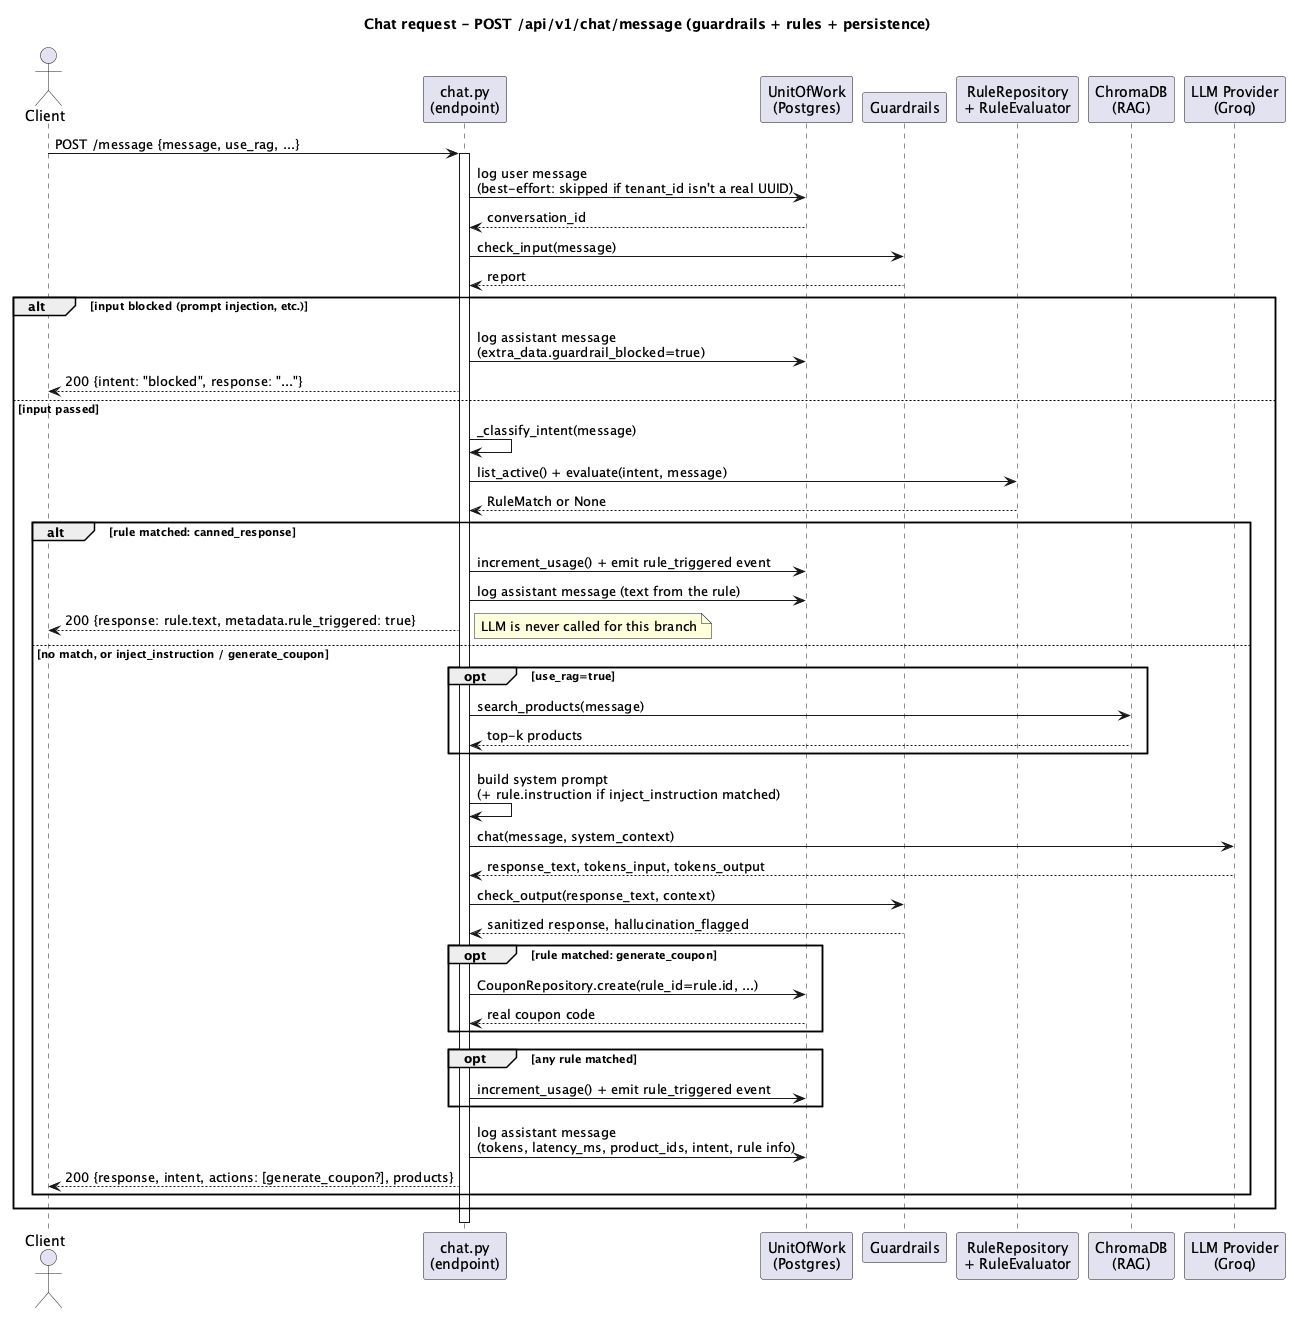
\includegraphics[width=\textwidth]{../diagrams/Sequence_Chat.png}
    \caption{Séquence complète d'une requête de chat}
    \label{fig:seq-chat}
\end{figure}

\section*{Conclusion}
\addcontentsline{toc}{section}{Conclusion}

Ce chapitre a présenté l'architecture retenue pour la plateforme ainsi que la modélisation des mécanismes centraux du système. Le chapitre suivant décrit la réalisation de ces éléments, sprint par sprint.
